\documentclass[a4paper,11pt]{article}
\usepackage[utf8]{inputenc}
\usepackage{algorithmic}
\usepackage{algorithm}
\usepackage{pst-plot}
\usepackage{graphicx}
\usepackage{endnotes}
\usepackage{graphics}
\usepackage{floatflt}
\usepackage{wrapfig}
\usepackage{amsfonts}
\usepackage{amsmath}
\usepackage{verbatim}
\usepackage{hyperref}
\usepackage{multirow}
\usepackage{pdflscape}

\usepackage{hyperref}
\hypersetup{pdfborder={0 0 0 0}}

\pdfpagewidth 210mm
\pdfpageheight 297mm 
\setlength\topmargin{0mm}
\setlength\headheight{0mm}
\setlength\headsep{0mm}
\setlength\textheight{250mm}	
\setlength\textwidth{159.2mm}
\setlength\oddsidemargin{0mm}
\setlength\evensidemargin{0mm}
\setlength\parindent{7mm}
\setlength\parskip{0mm}

\newenvironment{exercise}[3]{\paragraph{Exercise #1: #2 (#3pt)}\ \\}{
\medskip}
\newcommand{\question}[2]{\setlength\parindent{0mm}\ \\$\mathbf{Q_{#1}:}$ #2\ \\}


\author{\large{Ilya Kuzovkin, Raul Vicente}}
\title{\huge{Introduction to Computational Neuroscience}\\\LARGE{Practice I: Structure of the Brain}}

\begin{document}
\maketitle

As you might have heard before, structure of the brain is extremely complex. There are lots of neurons next to each other, tangled with each other, forming one, almost gapless mass. In pursuit of understanding any complex system, one thing you try to learn is its structure. Once you see the structure, you get insights about the purpose of the system. Same, hopefully, stands for our brain. Brain structure consist of neurons, their \emph{dentrites} (input channes), \emph{axons} (output channes) and \emph{synapses} (connections points). Eventually we would like to see this system in some structured and normalized form. The whole map of the brain (or part of it) is called \emph{connectome}. Building a connectome might reveal an information essential for understanding the inner workings of that part. 

\begin{exercise}{1}{EyeWire}{0.5}
One project aimed at creating a connectome of human brain is called EyeWire\footnote{\url{http://www.eyewire.org}}. The idea is similar to FoldIt\footnote{\url{http://fold.it}} or GalaxyZoo\footnote{\url{http://www.galaxyzoo.org}}: use human abilities and processing power to solve tasks where artificial intelligence fails. Read about this project's goals and motivation and start playing. In order to get points for this exercise complete the tutorial (first 6 cubes) and submit screenshot like the one below.
\begin{figure}[htbp]
   \centering
   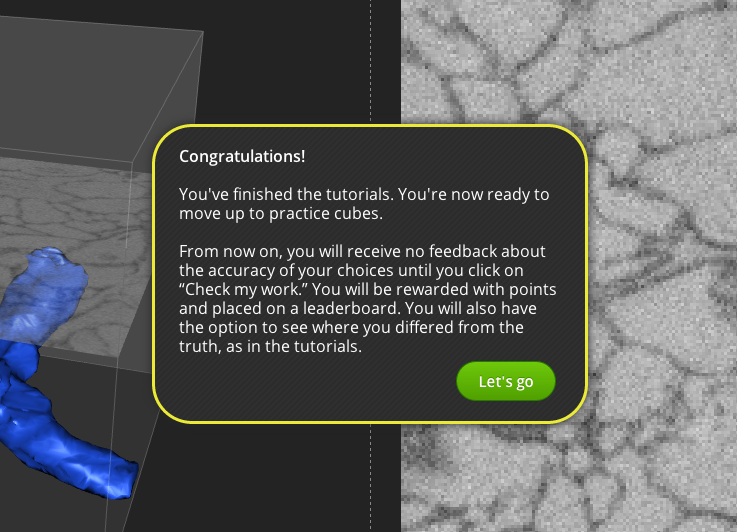
\includegraphics[width=0.5\textwidth]{eyewire.png} 
\end{figure}
\end{exercise}

\begin{exercise}{2}{Questionnaire}{1}
\question{1}{How many neurons are in the brain of a human, ant, bee, cat, caenorhabditis elegans, elefant?}
\question{2}{How many synapses are in the human brain?}
\question{3}{What is the main objective of the Human Brain Project?}
\question{4}{Describe the three levels of investigation by David Marr (top-down approach in neuroscience).}
\question{5}{Name 3 tasks at which computer is much better that human brain and 3 tasks where human brain outperforms any existing computer.}
\question{6}{What Aristotle thought the main function of the brain is?}
\question{7}{Describe the main function of the three main compartments of a neuron: soma, dendrite, axon.}
\question{8}{What is the main difference between grey and white matter?}
\question{9}{What is the main role of glial cells?}
\question{10}{Why is the cerebrum folded and convoluted?}
\question{11}{What do the following notions refer to: depolarization, repolarization, hyperpolarization?}
\question{12}{Which ionic pump is responsible for keeping negative resting membrane potential?}
\question{13}{In which sense action potentials are binary?}
\question{14}{If you were to flick a whale's tale then how long it will take for a while to realize that (compare myelinated and unmyelinated axonal transmission)?}
\question{15}{What is a neurotransmitter?}
\question{16}{Describe temporal and spatial summation.}
\end{exercise}

\begin{exercise}{3}{Types of neurons}{1.5}
There are lots of different types of neurons in our nervous system. They have different size, structure and function. Let us have a look at some of them:\\
\ \\
\begin{tabular}{p{3.7cm} p{3.7cm} p{3.7cm} p{3.7cm}}
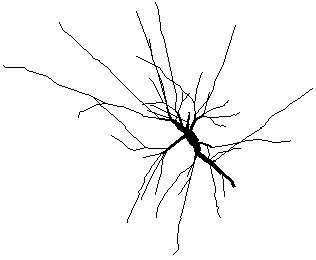
\includegraphics[width=0.25\textwidth]{pyramidal2.png} &
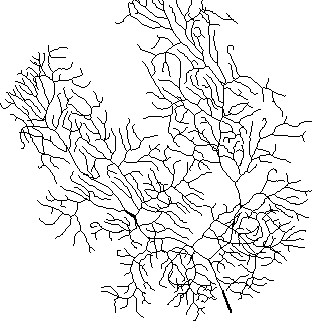
\includegraphics[width=0.25\textwidth]{purkinje.png} &

\includegraphics[height=0.25\textwidth]{spindle.png} &
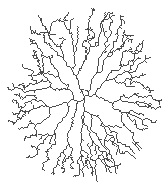
\includegraphics[width=0.25\textwidth]{amacrine.png}\\

\begin{center}\textbf{Pyramidal cell in layer 2 or 3}\end{center}&
\begin{center}\textbf{Purkinje cell}\end{center}&
\begin{center}\textbf{Spindle neuron}\end{center}&
\begin{center}\textbf{Amacrine cell}\end{center} \\
\end{tabular}
\begin{tabular}{p{3.7cm} p{3.7cm} p{3.7cm} p{3.7cm}}
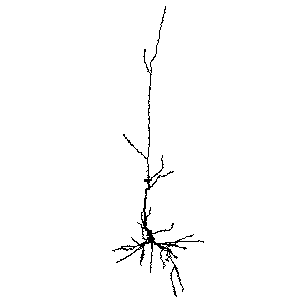
\includegraphics[width=0.25\textwidth]{pyramidal5.png} &
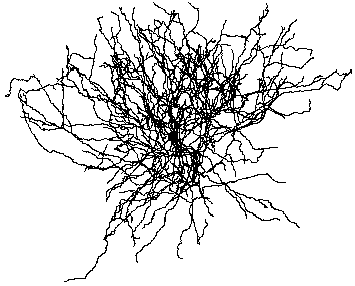
\includegraphics[width=0.25\textwidth]{bascet.png} &
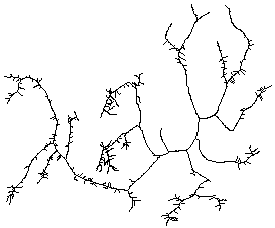
\includegraphics[height=0.25\textwidth]{sensory.png} &
 \\

\begin{center}\textbf{Pyramidal cell in layer 5}\end{center}&
\begin{center}\textbf{Basket cell}\end{center}&
\begin{center}\textbf{Sensory neuron}\end{center}&
\begin{center}\textbf{}\end{center} \\
\end{tabular}


In the \texttt{data} folder of this assignment you will find three \texttt{.swc} files. Each file describes reconstructed structure of a neuron. Neuron can be classified by different parameters, such as size, bifurcation, size of some, etc. In general task of identifying type of a neuron is quite hard\footnote{M. Bota, L. W. Swanson, \textbf{The neuron classification problem}, 2007, 
\url{http://www.sciencedirect.com/science/article/pii/S0165017307000768}}. But when looked at, different types of neurons have distinguishable shapes. This is what we will try to use in this exercise. Your task is to plot neurons from the data files and guess which of the above-mentioned types each of them belongs to.
\begin{enumerate}
	\item Have a look inside an \texttt{.swc} file. Each line describes small piece of the neuron (\emph{compartment}), space-separated values are: 
	\begin{enumerate}
		\item ID of the compartment
		\item Type of the compartment:
		\begin{enumerate}
			\item[0] -- undefined
			\item[1] -- soma
			\item[2] -- axon
			\item[3] -- basal dendrite
			\item[4] -- apical dendrite
		\end{enumerate}
		\item X coordinate (in $\mu$m)
		\item Y coordinate
		\item Z coordinate	
		\item Radius of the compartment
		\item ID of parent compartment (-1 for root compartment)
	\end{enumerate}
	\item Import coordinate data into your program (or \texttt{Matlab}, \texttt{R} environment)
	\item Plot data in 3D (for example using \texttt{scatter3} in \texttt{Matlab})
	\item Look at resulting 3D image an try to guess type of the neuron
\end{enumerate}
\ \\
In your report please tell type of the neuron for each of the files, include visualizations and the code to reproduce them. You can use \texttt{Matlab/Octave}, \texttt{R}, \texttt{Python} or any other programming language. During the course we consider \texttt{Matlab} to be our primal tool, so if you don't have any strong preferences, try using \texttt{Matlab/Octave}.
\end{exercise}

\begin{exercise}{4}{Brain lesions}{0.5}
Brain \emph{lesions} are abnormalities in the structure of the brain. Some lesions lead to interesting effects, that give us information about functional role of the damaged region. Read about brain lesions and possible effects. Google up one lesion, which triggers your interest and:
\begin{itemize}
\itemsep 0em
	\item describe the nature of the lesion
	\item find a picture of the structure it appears in
	\item tell about its characteristics, e.g. is it temporal or permanent
	\item describe the effect it causes
	\item speculate on how the effect is related to the functional role of that region
\end{itemize}
\end{exercise}
\ \\
\ \\
\ \\
\ \\
\ \\
Please submit a \texttt{pdf} report with answers to the questions and comments about your solutions. Also submit the code for the programming exercise(s). Pack those into \texttt{zip} archive and upload to the course web page.

\end{document}










